\setcounter{section}{0}
\renewcommand{\thesection}{\Alph{section}}%
% TODO: MOVE TO THE APPENDICES
\section{Correctness proof} \label{App:proofs}

This Appendix provides a proof that when \solveCHC\ returns SAFE, no feasible path $\route^\top_\bot$ exists through the CHC system.
For this purpose, we introduce the notion of \emph{concise} expansions and several supporting lemmas.

\begin{definition}[Concise expansion of a simple path]
Given a CHC system $\system$ over a set of uninterpreted predicates $\preds$ with uninterpreted predicates 
$\sourcepred, \targetpred \in \preds$, a simple path $\proute^{\sourcepred}_{\targetpred} = [\clause_1, \dots, \clause_n]$  and a set of predicates 
$\preds_e = \{\pred_1, \dots, \pred_n\} \subset \predsf(\proute^{\sourcepred}_{\targetpred})$, a concise expansion of the simple path is a new path: 
$\cexp(\proute^{\sourcepred}_{\targetpred}, \preds_e) = [\clause_1, \dots, \clause_{i-1}] \oplus \route^{\pred_i}_{\pred_i} \oplus 
[\clause_i, \dots, \clause_{j-1}] \oplus \route^{\pred_j}_{\pred_j} \oplus [\clause_j, \dots, \clause_n]$, where
for every $\route^{\pred}_{\pred}$ in $\cexp(\proute^{\sourcepred}_{\targetpred}, \preds_e)$ the following holds
$\predsf(\route^{\pred}_{\pred}) \cap (\predsf(\proute^{\sourcepred}_{\pred}) \setminus \{\pred\}) = \emptyset$, 
where $\proute^{\sourcepred}_{\pred} \subseteq \proute^{\sourcepred}_{\targetpred}$.
If $\preds_e = \emptyset$, then $\cexp(\proute^{\sourcepred}_{\targetpred}, \preds_e) = \proute^{\sourcepred}_{\targetpred}$.
\end{definition}

We call cycle path $\route_\pred^\pred$ \emph{concise} with respect to $\preds_b$ if 
$\predsf(\route_\pred^\pred) \cap \preds_b = \emptyset$. 
\textbf{All cycle paths constructed by} \queryUnrolling \textbf{are concise}, with respect to the 
predicates $\predsf(\proute^{\top}_{\pred}) \setminus \{\pred\}$ for any 
call to \summarize.


\begin{example}
\begin{subfigures}
%
\begin{figure}[!ht]
   \begin{minipage}{0.35\textwidth}
        \centering
        {
            \scriptsize
            \begin{align*}
                \phi_1(x)& \implies \pred_1(x) &&\clause_1\\
                \phi_2(x) &\implies \pred_2(x) &&\clause_2\\
                \pred_1(x) \land \phi_3(x,x') &\implies \pred_2(x') &&\clause_3\\
                \pred_2(x) \land \phi_4(x,x') &\implies \pred_1(x') &&\clause_4\\
                \pred_2(x) \land \phi_5(x,x') &\implies \bot &&\clause_5
            \end{align*}
        }
        \caption{CHC system}\label{fig:chcConc}
    \end{minipage}\hfill
    \begin{minipage}{0.65\textwidth}
        \centering
        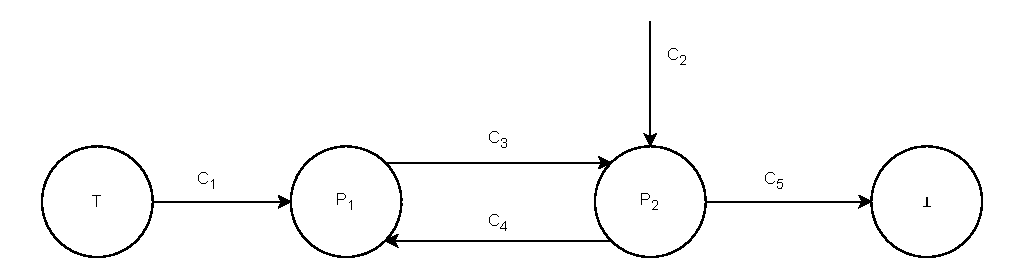
\includegraphics[width=1\textwidth]{Figures/ConciseEx.pdf}
        \caption{Graph representation of CHC System~\ref{fig:chcConc}}
   \end{minipage}
\end{figure}

\end{subfigures}

Consider the CHC system in Figure~\ref{fig:chcConc}. 
This system contains two simple paths from $\top$ to $\bot$: $\proute_1 = [\clause_1, \clause_3, 
\clause_5]$ and $\proute_2 = [\clause_2, \clause_5]$. 
A concise expansion of $\proute_1$ over $\pred_1$ with respect to the prefix simple path
$\proute_{\pred_1}^\top = [\clause_1]$ would look like: $\cexp(\proute_1, \{\pred_1\}) = [\clause_1]  
\oplus \route_{\pred_1}^{\pred_1} \oplus [\clause_3, \clause_5]$
Here, $\route_{\pred_1}^{\pred_1}$ consists of one or more iterations of the cycle $[\clause_3, \clause_4]$.
However, for $\proute_1$, a concise expansion over predicate $\pred_2$ does not exist. 
This is because cycles over $\pred_2$ are formed by $\iteration_{\pred_2}^{\pred_2} = 
[\clause_4, \clause_3]$, but $\predsf([\clause_4, \clause_3]) \cap \predsf([\clause_1, \clause_3]) = 
\{\pred_1, \pred_2\}$. 
This violates the conciseness condition.
In contrast, a concise expansion of $\proute_2$ over $\pred_2$ does exist, since 
$\predsf(\route_{\pred_2}^{\pred_2}) \cap \predsf([\clause_2]) = \{\pred_2\}$. 
Therefore, $\cexp(\proute_2, \{\pred_2\}) = [\clause_2] \oplus \route_{\pred_2}^{\pred_2} \oplus 
[\clause_5]$ is a concise expansion.
\end{example}

It possible to prove that any possible path through the CHC system is a simple path or concise expansion of a 
simple path.

\begin{lemma}[Concise predicate expansions]\label{Lem:concise}
    Given a CHC system $\system$ over predicates $\preds$, $\sourcepred, \targetpred \in \preds$, any
    path $\route_{\targetpred}^{\sourcepred}$ is either a simple path 
    $\proute_{\targetpred}^{\sourcepred}$, or a concise expansion of a simple path 
    $\route_{\targetpred}^{\sourcepred} = \cexp(\proute_{\targetpred}^{\sourcepred}, [\dots])$.
\end{lemma}

\begin{proof}
    We prove this lemma by induction on the length of the path $\route_{\targetpred}^{\sourcepred}$.

    %

    \textbf{Base case}: If $|\route_{\targetpred}^{\sourcepred}| = 1$, then the path consists of a 
    single clause $\clause^{\sourcepred}_{\targetpred}$. By definition, this is a simple path.

    %

    \textbf{Inductive case}: Assume the lemma holds for all paths of length $n$. Consider a path of 
    length $n+1$ formed by appending a clause $\clause_{\pred}^{\targetpred}$ to an existing 
    path $\route^\sourcepred_\targetpred$ of length $n$.  It is sufficient to only consider adding a 
    clause to the end of $\route^\sourcepred_\targetpred$.

    %

    Let us consider a path of size $n$:
        $[\clause_1, \dots, \clause_{n-1}, \clause_n]$. 
    If clause $\clause$ is added in the beginning (or in the middle) of it, we get a new path:
        $[\clause, \clause_1, \dots, \clause_{n-1}, \clause_n]$. 
    By our inductive assumption all paths of size $n$ are either concise expansions of simple 
    paths or simple paths, then $[\clause, \clause_1, \dots, \clause_{n-1}]$ is a concise 
    expansion or a simple path. 
    Therefore it is the same problem as adding $\clause_n$ to simple path or concise expansion 
    $[\clause, \clause_1, \dots, \clause_{n-1}]$, and it is sufficient to consider only the case
    when $\clause$ is added to the end of the path.

    %

    We consider two cases, depending on whether the initial path $\route^\sourcepred_\targetpred$ 
    is a simple path or a concise expansion of a simple path.

    %

    \textbf{Case 1}: Let us consider appending a clause $\clause_{\pred}^{\targetpred}$ to the simple path
    $\proute_{\targetpred}^{\sourcepred}$. 
    There are two sub-cases:
    \begin{itemize}
        \item If $\forall \clause \in \proute_{\targetpred}^{\sourcepred}$: $\source(\clause) \neq 
            \targetpred$ and $\target(\clause) \neq \pred$, then the extended path remains a simple 
            path: $\proute^\sourcepred_\pred = \proute^\sourcepred_\targetpred \oplus 
            [\clause^\targetpred_\pred]$.
        \item Otherwise, appending $\clause$ would introduce a cycle. There are two possibilities:
        \begin{itemize}
            \item $\exists \clause \in \proute_{\targetpred}^{\sourcepred}$ such that 
                $\source(\clause) = \targetpred$. This can happen only if $\sourcepred = \targetpred$. 
                Otherwise, path would contain clauses $\clause_\targetpred^*, \clause^\targetpred_*$ 
                and the last clause is also $\clause_\targetpred^*$, which contradicts definition of a
                simple path (since there would exist multiple clauses in $\proute^\sourcepred_\targetpred$
                such that $\target(\clause) = \targetpred$). 
                In this case, the extended path becomes 
                $\proute_{\targetpred}^{\targetpred} \oplus [\clause^{\targetpred}_{\pred}]$, which 
                is a concise expansion: $\cexp([\clause^{\targetpred}_{\pred}], \{\targetpred\})$.  
            \item $\exists \clause \in \proute_{\targetpred}^{\sourcepred}$ such that 
                $\target(\clause) = \pred$. Then, the simple path can be written as 
                $\proute_{\targetpred}^{\sourcepred} = \proute_{\pred}^{\sourcepred} \oplus 
                \proute_{\targetpred}^{\pred}$, and the extended path becomes  $\proute^\sourcepred_\pred 
                \oplus \proute^\pred_\targetpred \oplus [\clause^\targetpred_\pred]$, where 
                $\proute_{\targetpred}^{\pred} \oplus [\clause_{\pred}^{\targetpred}] = 
                \route_{\pred}^{\pred}$ forms a cycle. Since $\predsf(\route_{\pred}^{\pred}) \cap
                \predsf(\proute_{\pred}^{\sourcepred}) = \{\pred\}$, the new path is a concise 
                expansion: $\cexp(\proute_{\pred}^{\sourcepred}, \{\pred\})$.
        \end{itemize}
    \end{itemize}

%

    \textbf{Case 2}: Let us consider appending $\clause_{\pred}^{\targetpred}$ to a concise
    expansion $\route_{\targetpred}^{\sourcepred} = \cexp(\proute_{\targetpred}^{\sourcepred}, \{\dots\})$.
    This means the path can be written as:
    \[
        \route_{\targetpred}^{\sourcepred} = \route_{\sourcepred}^{\sourcepred} \oplus 
        [\clause^{\sourcepred}_{*}] \oplus \dots \oplus [\clause^{*}_{\targetpred}] \oplus 
        \route_{\targetpred}^{\targetpred}
    \]
    where each cycle $\route_{\sourcepred}^{\sourcepred}, \dots,\route_{\targetpred}^{\targetpred}$ is
    concise with respect to the corresponding simple prefix $\emptyset, \dots, 
    \proute_{\targetpred}^{\sourcepred} \subseteq \proute_{\targetpred}^{\sourcepred}$.

    \begin{itemize}
        \item If $\forall \clause \in \proute_{\targetpred}^{\sourcepred}$: 
            $\source(\clause) \neq \targetpred$ and $\target(\clause) \neq \pred$, then the 
            resulting path remains a concise expansion $\cexp(\proute_{\pred}^{\sourcepred}, \{\dots\})$
            of a longer simple path $\proute_{\pred}^{\sourcepred} = \proute_{\targetpred}^{\sourcepred}
            \oplus [\clause_{\pred}^{\targetpred}]$ over same predicates.
        \item Otherwise, as in the simple path case, two situations may occur:
        \begin{itemize}
            \item $\exists \clause \in \proute_{\targetpred}^{\sourcepred}$ such that 
                $\source(\clause) = \targetpred$. This again implies $\sourcepred = \targetpred$, 
                and the path can be rewritten as $\cexp([\clause^{\targetpred}_{\pred}], \{\targetpred\})$.
            \item$\exists \clause \in \proute_{\targetpred}^{\sourcepred}$ such that 
                $\target(\clause) = \pred$. The original path can be rewritten as:
                \[
                    \route_{\targetpred}^{\sourcepred} = \route^\sourcepred_\sourcepred \oplus 
                    [\clause^\sourcepred_*] \oplus \dots \oplus [\clause^*_\pred] \oplus 
                    \route_\pred^\pred \oplus  [\clause_*^\pred]\oplus \dots \oplus 
                    [\clause^*_\targetpred] \oplus \route^\targetpred_\targetpred
                \]
                When clause $\clause_\pred^\targetpred$ is added to $\route_{\targetpred}^{\sourcepred}$,
                then $(\route_\pred^\pred \oplus  [\clause_*^\pred]\oplus \dots 
                \oplus [\clause^*_\targetpred] \oplus \route^\targetpred_\targetpred) 
                \oplus \clause_\pred^\targetpred$ forms a cycle $\route_\pred^\pred$, 
                and overall path can be rewritten as follows:
                \[
                \route_{\targetpred}^{\sourcepred} = \route_{\sourcepred}^{\sourcepred} \oplus 
                    [\clause^{\sourcepred}_{*}] \oplus \dots \oplus [\clause^{*}_{\pred}] \oplus 
                    \route_{\pred}^{\pred}
                \]
            where $\predsf(\route_{\pred}^{\pred}) \cap \predsf(\proute_{\pred}^{\sourcepred}) = 
            \{\pred\}$. Therefore the resulting path is a concise expansion: 
            $\cexp(\proute_{\pred}^{\sourcepred}, \{\dots, \pred\})$ where 
            $\proute_{\pred}^{\sourcepred} \subseteq \proute_{\targetpred}^{\sourcepred}$ is simple prefix.

        \end{itemize}
        
    \end{itemize}
    
    By structural induction, we have shown that any path is either a simple path or a concise 
    expansion of a simple path.
\end{proof}

\begin{lemma}[Iteration Overapproximation]\label{Lem:mu}
    Let \emph{\mergeTransition} called over a CHC system $\system$, a set of blocked predicates $\preds_b$,
    a map of summaries $\summaries$, 
    and a predicate $\pred$, return a formula $\mu$. 
    Then, for any iteration path $\iteration_\pred^\pred$ such that $\iteration_\pred^\pred \cap 
    \preds_b = \emptyset$:
    $\encoding(\iteration_\pred^\pred)(x^{(0)}, \dots, x^{(n)}) \implies \mu(x^{(0)}, \dots, x^{(n)}).$
\end{lemma}

\begin{proof}
    Let us prove this lemma by contradiction. Assume there exists an iteration path 
    $\iteration^\pred_\pred$ such that $\iteration^\pred_\pred \cap \preds_b 
    = \emptyset$ and $\encoding(\iteration^\pred_\pred)(x^{(0)}, \dots, x^{(n)}) \land \lnot 
    \mu(x^{(0)}, \dots, x^{(n)})$ is satisfiable. 

    By Lemma~\ref{Lem:concise}, any path $\iteration^\pred_\pred$ is either 
    a simple path $\proute_\pred^\pred$, or a concise expansion of a simple path
    $\proute_\pred^\pred = [\clause_1, \dots, \clause_m]$. 
    Therefore, the iteration can be written as $\iteration_\pred^\pred = \cexp(\proute_\pred^\pred, 
    \dots)$ = $[\clause_1] \oplus \route^{\source(\clause_2)}_{\source(\clause_2)} \oplus [\clause_2] 
    \oplus \dots  \oplus \route^{\source(\clause_m)}_{\source(\clause_m)} \oplus \clause_m$ 
    where each cycle path $\route^{\source(\clause)}_{\source(\clause)}$ for 
    $\clause \in \proute_\pred^\pred$ is either an empty path or a concise
    cycle path with respect to $\predsf(\proute^\pred_{\source(\clause)}) \setminus \source(\clause)$. 
    Importantly, there are no cycle paths $\route^{\pred}_{\pred}$ present in $\iteration^\pred_\pred$
    ($\route^{\source(\clause_1)}_{\source(\clause_1)}$ and 
    $\route^{\target(\clause_m)}_{\target(\clause_m)}$), since otherwise 
    $\iteration^\pred_\pred$ would not be an iteration path.
    If for every clause $\clause \in \proute_\pred^\pred$ corresponding cycle path 
    $\route^{\source(\clause)}_{\source(\clause)}$ in $\iteration_\pred^\pred$ is empty, then 
    $\iteration_\pred^\pred$ is a simple path.
    
    As described in Subsection~\ref{Section:Summarize}, $\mu = \bigvee \mu_{\proute}$, where each 
    $\mu_{\proute}$ corresponds to a specific simple path $\proute_\pred^\pred$. 
    By our initial assumption, $\encoding(\iteration^\pred_\pred) \land \lnot \mu$ is satisfiable,
    so $\encoding(\iteration^\pred_\pred) \land \lnot \mu_{\proute}$
    is also satisfiable for every $\mu_{\proute}$.
    Let us consider specifically $\mu_{\proute}$, which was constructed for the same simple path as used 
    in the considered iteration $\iteration^\pred_\pred = \cexp(\proute_\pred^\pred, \dots)$. 
    The conjunction $\encoding(\iteration^\pred_\pred) \land \lnot \mu_{\proute}$ can be 
    written as:
    {\footnotesize
    \begin{align*}
        \encoding(\iteration^\pred_\pred)&(x^{(0)}, \dots, x^{(n)}) \land \lnot 
            \mu_{\proute}(x^{(0)}, \dots, x^{(n)}) = \\
        ( \\
        & \constraint(\clause_1)(x^{(0)}, x^{(1)})\ \land  && (\clause_1) \\ 
        & \big(\encoding(\route_{\source(\clause_2)}^{\source(\clause_2)})(x^{(1)}, \dots, x^{(i)}) 
            \land \constraint(\clause_2)(x^{(i)}, x^{(i+1)})\big)\ \land   && (\clause_2) \\ 
        & \dots\ \land \\ 
        & \big(\encoding(\route_{\source(\clause_m)}^{\source(\clause_m)})(x^{(j)}, \dots, x^{(n-1)})
            \land \constraint(\clause_m)(x^{(n-1)}, x^{(n)})\big)  && (\clause_m) \\
        ) \land \lnot ( \\
        &  \constraint(\clause_1)(x^{(0)}, x^{(1)}) \land  && (\clause_1)\\
        & \big(\constraint(\clause_2)(x^{(1)}, x^{(i+1)}) \lor 
            (\summaries(\source(\clause_2), \preds_b)(x^{(1)}, x^{(i)}) \land 
            \constraint(\clause_2)(x^{(i)}, x^{(i+1)}))\big)\ \land  && (\clause_2)\\
        & \dots\ \land \\
        & \big(\constraint(\clause_m)(x^{(j)}, x^{(n)}) \lor  
            (\summaries(\source(\clause_m),  (\predsf(\proute) \setminus \{\source(\clause_m)\}) \cup 
            \preds_b)(x^{(j)}, x^{(n-1)}) && (\clause_m)\\ 
        &   \land \constraint(\clause_m)(x^{(n-1)}, x^{(n)})) \big)  \\
        ).
    \end{align*}
    }
    The formula $\encoding(\iteration^\pred_\pred)(x^{(0)}, \dots, x^{(n)}) \land \lnot 
    \mu_{\proute}(x^{(0)}, \dots, x^{(n)})$ is unsatisfiable. To prove it, let us show that 
    $\encoding(\iteration^\pred_\pred)(x^{(0)}, \dots, x^{(n)})$ is UNSAT when conjoined with negation
    of any conjunct in $\mu_{\proute}$. 
    
    As demonstrated above, every conjunct in 
    $\encoding(\iteration^\pred_\pred)$ and in $\mu_{\proute}$ can be mapped to the specific clause 
    $\clause_i \in \proute^\sourcepred_\targetpred$ (in the column on the right). 
    By conjoining conjuncts in $\encoding(\iteration^\pred_\pred)$ with the negations of corresponding
    conjuncts in $\mu_{\proute}$ is is possible to demonstrate that $\encoding(\iteration^\pred_\pred)(x^{(0)}, 
    \dots, x^{(n)}) \land \lnot \mu_{\proute}(x^{(0)}, \dots, x^{(n)})$ is unsatisfiable.

    First, consider the case of $\encoding(\iteration^\pred_\pred)(x^{(0)}, \dots, x^{(n)}) \land 
    \lnot \constraint(\clause_1)(x^{(0)}, x^{(1)})$. This is trivially unsatisfiable since 
    $\constraint(\clause_1)(x^{(0)}, x^{(1)})$ is a conjunct in $\encoding(\iteration^\pred_\pred)$.

    Now, consider any conjunct $conj_\mu$ in $\mu_\proute$ mapped to 
    some clause $\clause_i \in \proute_\pred^\pred$, with $\source(\clause_i) = q$:
    $$conj_\mu(x^{(k)}, x^{(l)}, x^{(l+1)}) = (\summaries(q, \preds_b')(x^{(k)}, x^{(l)}) \land
    \constraint(\clause_i)(x^{(l)}, x^{(l+1)})) \lor \constraint(\clause_i)(x^{(k)}, x^{(l+1)}).$$    
    where $\preds_b'= \preds_b \cup \{\pred\} \cup (\predsf(\proute^\pred_{\source(\clause_i)}) \setminus \{\source(\clause_i)\})$ 
    and $\proute^\pred_{\source(\clause_i)} \subseteq \proute^\pred_\pred$.
    The corresponding conjunct $conj_{\iteration}$ in $\encoding(\iteration^\pred_\pred)$ is:
    $$conj_{\iteration}(x^{(k)}, \dots, x^{(l+1)}) =  (\encoding(\route_{q}^{q})(x^{(k)}, \dots, x^{(l)})
    \land \constraint(\clause_i)(x^{(l)}, x^{(l+1)})).$$
    And overall formula:
    \begin{align*}
        &conj_\iteration(x^{(k)}, \dots, x^{(l+1)}) \land \lnot conj_\mu(x^{(k)}, x^{(l)}, x^{(l+1)}) = \\ 
        &\big(conj_\iteration(x^{(k)}, \dots, x^{(l+1)}) \land 
            \lnot (\summaries(q, \preds_b')(x^{(k)}, x^{(l)}) \land 
            \constraint(\clause_i)(x^{(l)}, x^{(l+1)}))\big) \land \\
        &\big(conj_\iteration(x^{(k)}, \dots, x^{(l+1)}) \land 
            \lnot  \constraint(\clause_i)(x^{(k)}, x^{(l+1)})\big).
    \end{align*}
    % conj_\iteration \land \lnot conj_\mu = $$
    There are two cases for $conj_\iteration$. First, when $\route_{q}^{q} = \emptyset$, then
    $k = l$ and:
    $$conj_\iteration(x^{(k)}, x^{(l+1)}) = \constraint(\clause_i)(x^{(k)}, x^{(l+1)})$$
    Since $\constraint(\clause_i)(x^{(k)}, x^{(l+1)}) \land \lnot
    \constraint(\clause_i)(x^{(k)}, x^{(l+1)})$ is unsatisfiable, $conj_\iteration \land \lnot conj_\mu$ is 
    also unsatisfiable.

    %

    Otherwise, if $\route_{q}^{q} \neq \emptyset$, then by the definition of summary,
    $\encoding(\route_{q}^{q})(x^{(k)}, \dots, x^{(l)}) \land \lnot \summaries(q, \preds_b')(x^{(k)}, x^{(l)})$ 
    is unsatisfiable since $\route_{q}^{q}$ is concise with respect to $\preds_b'$. 
    Therefore, 
    \begin{align*}
    & \big((\encoding(\route_{q}^{q})(x^{(k)}, \dots, x^{(l)}) \land 
    \constraint(\clause_i)(x^{(l)}, x^{(l+1)})) \land \lnot \summaries(q, \preds_b')(x^{(k)}, x^{(l)}) \big)\ \lor \\
    & \big( (\encoding(\route_{q}^{q})(x^{(k)}, \dots, x^{(l)})
    \land \constraint(\clause_i)(x^{(l)}, x^{(l+1)})) \land \lnot \constraint(\clause_i)(x^{(l)}, x^{(l+1)})\big)
    \end{align*}
    $$$$
    is also unsatisfiable which means that $conj_\iteration \land \lnot conj_\mu$ is unsatisfiable.
    We've demonstrated that for every negation of conjunct $conj_\mu$ in $\mu_{\proute}$, the 
    conjunction $\encoding(\iteration^\pred_\pred) \land \lnot conj_\mu$ is unsatisfiable. 
    Which means that $\encoding(\iteration^\pred_\pred) \land \lnot \mu_{\proute}$ is unsatisfiable.
    It is a contradiction of initial assumption that $\encoding(\iteration^\pred_\pred) 
    \land \lnot \mu$ is satisfiable. This completes the proof.
\end{proof}

\begin{lemma}[Cycle summarization]\label{Lem:expSat}
    If \emph{\summarize}, invoked over CHC System $\system$ with a set of blocked predicates $\preds_b$ 
    and Pre/Post formulas $\precond, \postcond$, returns a tuple 
    $\tuple{\emptyset, \summaries}$, then no feasible cycle 
    path $\route_{\pred}^{\pred}$ with $\predsf(\route_{\pred}^{\pred}) \cap \preds_b = \emptyset$ exists, such 
    that $\precond(\dots, x) \land \encoding(\route_{\pred}^{\pred})(x, \dots, x') \land 
    \postcond(x')$ is satisfiable.
\end{lemma}

\begin{proof}
    We prove this lemma by contradiction. 
    Suppose there exists a cycle path 
    $\route_\pred^\pred$ with predicates $\predsf(\route_\pred^\pred) \cap \preds_b = \emptyset$ such 
    that $\precond(\dots, x) \land \encoding(\route_{\pred}^{\pred})(x, \dots, x') \land 
    \postcond(x')$ is satisfiable. 

    Any possible cycle path can be decomposed into multiple iteration paths $\iteration^\pred_\pred$: 
    $\route_\pred^\pred = \iteration_1 \oplus \dots \oplus \iteration_n$. 
    Therefore the path condition can be written as 
    $\encoding(\route_\pred^\pred)(x, \dots, x') = \encoding(\iteration_1)(x, \dots, x^{(i)}) \land \dots 
    \land \encoding(\iteration_n)(x^{(j)}, \dots, x')$. 
    
    \summarize, at Line~\ref{summarize:mtr}, constructs formula $\mu$ to overapproximate 
    all possible iteration paths.
    By construction (Lemma~\ref{Lem:mu}), for any iteration path $\iteration$ with $\predsf(\iteration)
    \cap \preds_b = \emptyset$, it holds that $\encoding(\iteration)(x, \dots, x') \implies 
    \mu(x, \dots, x')$.  
    Thus, $\encoding(\iteration_1)(x, \dots, x^{(i)}) \land \dots \land 
    \encoding(\iteration_n)(x^{(j)}, \dots, x') \implies \mu(x, \dots, x^{(i)}) 
    \land \dots \land \mu(x^{(j)}, \dots, x')$, where each $\encoding(\iteration_i)$ is mapped to 
    a corresponding $\mu$.
    It means that $\precond(\dots, x) \land  \mu(x, \dots, x^{(i)}) 
    \land \dots \land \mu(x^{(j)}, \dots, x') \land \postcond(x')$ is also satisfiable.

    Additionally, by the definition of \tpa which returned $\tuple{\emptyset, \summary_\pred}$, 
    $\mu(x, \dots, x^{(i)}) \land \dots \land \mu(x^{(j)}, \dots, x') \implies \summary_\pred(x,x')$.
    Thus, $\precond(\dots, x) \land \summary_\pred(x, x') \land \postcond(x')$ is
    satisfiable.
    However, by same definition of \tpa $\precond(\dots, x) \land \summary_\pred(x, x') 
    \land \postcond(x')$ is unsatisfiable. 
    This is a contradiction. 
    Therefore, a path $\route_\pred^\pred$ does not exist.
\end{proof}

\begin{lemma}[Pre and Post formulas]~\label{Lem:encodings}
    \emph{\queryUnrolling} \textbf{invariant:}
    Suppose \emph{\queryUnrolling} is called over CHC system $\system$ with blocked predicates 
    $\preds_b$, map of cycle summaries $\summaries$, and Pre, Post formulas 
    $\precond, \postcond$  over a simple path $\proute_\bot^\top$ . 
    For any $\clause_i \in \predsf(\proute_\bot^\top)$, $\source(\clause_i) = \pred$
    there does not exist a feasible concise expansion $\cexp(\proute_\bot^\top, \{\dots, \pred, \dots\}) = 
    \route^{\top}_{\pred} \oplus \route^{\pred}_{\pred} \oplus \route^{\pred}_{\bot}$ 
    such that either of the following formulas is satisfiable: 
    \begin{align*}
        &\encoding(\route^{\top}_{\pred})(x,\dots,x') \land 
            \lnot \precond(\clause_{i})(x') \land \encoding(\route^{\pred}_{\pred} \oplus 
            \route^{\pred}_{\bot})(x', \dots, x'') \\
        &\encoding(\route^{\top}_{\pred} \oplus 
            \route^{\pred}_{\pred})(x,\dots,x') \land \lnot \postcond(\clause_{i})(x') \land 
            \encoding(\route^{\pred}_{\bot})(x',\dots,x'') 
    \end{align*}
\end{lemma}

\begin{proof}
    We prove this lemma by induction. 
    
    \textbf{Base case:} Initially, for all $\clause_i \in \proute_\bot^\top$, 
    both $\precond(\clause_{i})$ and $\postcond(\clause_{i})$  are set to $\top$, so the invariant holds 
    trivially.

    %

    \textbf{Inductive case:} Assume the invariant holds at some point during the execution.
    Pre and Post formulas $\precond(\clause_{i}),\postcond(\clause_{i})$ may be updated at 
    Lines~\ref{queryUnrolling:postcondupd}, \ref{queryUnrolling:precondF}, and 
    \ref{queryUnrolling:precondupd} of Algorithm~\ref{Alg:QueryUnrolling}. 


    %

    On Line~\ref{queryUnrolling:postcondupd}, the algorithm updates $\postcond(\clause_{i})$ when 
    extending the path with a clause from the original simple path $\clause_i \in \proute^{\top}_{\bot}$, 
    $\source(\clause_i) = \pred$.
    The update at Line~\ref{queryUnrolling:postcondupd} 
    maintains following relation by construction: $\lnot \postcond(\clause_i)(x) 
    \land \constraint(\clause_i)(x,x') \implies \lnot \precond(\clause_{i+1})(x')$. 
    Since for $\lnot \precond(\clause_{i+1})$ invariant holds, then it also holds for 
    $\postcond(\clause_i)$.

    %

    On Line~\ref{queryUnrolling:precondF}, the precondition $\precond(\clause_i)$ is strengthened based 
    on the cycle summary $\summaries(\pred, \preds_b)$. For any concise cycle path $\route^i_i$
    following formula $\lnot \precond(\clause_i)(x) \land \route^i_i(x,x') \land 
    \postcond(\clause_i)(x')$ is UNSAT (based on the definition of cycle summary).
    Therefore,  $\lnot \precond(\clause_i)(x) \land \summaries(\pred, \preds_b)(x,x') \implies \lnot 
    \postcond(\clause_i)(x')$. 
    Since $\encoding(\route^{\sourcepred}_{\pred} \oplus 
            \route^{\pred}_{\pred})(x,\dots,x') \land \lnot \postcond(\clause_i)(x') \land 
            \encoding(\route^{\pred}_{\targetpred})(x',\dots,x'')$ is unsatisfiable,
    invariant still holds for $\precond(\clause_i)$.
    % Since $\encoding(\route^{\sourcepred}_{\pred} \oplus 
    %         \route^{\pred}_{\pred})(x,\dots,x') \land \lnot \postcond_i(x') \land 
    %         \encoding(\route^{\pred}_{\targetpred})(x',\dots,x'')$ is 
    % unsatisfiable, and for new $\precond_\pred$ it holds that  $\lnot \precond_\pred(x) \land 
    % \summaries(\pred, \preds_b)(x,x') \implies \lnot \postcond_\pred(x')$, thus, 
    % $\encoding(\route^{\sourcepred}_{\pred})(x,\dots,x') \land 
    %         \lnot \precond_{i}(x') \land \encoding(\route^{\pred}_{\pred} \oplus 
    %         \route^{\pred}_{\targetpred})(x', \dots, x'') $ is also unsatisfiable.
    
    %

    Finally, on Line~\ref{queryUnrolling:precondupd} Pre formula $\precond(\clause_i)$ is updated as
    $\precond(\clause_i) \gets \postcond(\clause_i)$, which preserves the invariant since concise cycle 
    over $\pred$ does not exist.
    Therefore, in all cases, the updates to $\precond(\clause_i)$ and $\postcond(\clause_i)$ preserve the 
    invariant.
\end{proof}


The proof for \textbf{Theorem}~\ref{Thm:SAT} is given below.

\begin{proof}
    The proof follows from Lemma~\ref{Lem:encodings} and Lemma~\ref{Lem:concise}. 
    Algorithm~\ref{Alg:solveCHC} invokes \queryUnrolling to determine whether any simple 
    path $\proute^\top_\bot$ in the CHC system can be expanded into a satisfiable path. 
    \queryUnrolling returns $\emptyset$ only when it enters "if" at 
    Line~\ref{queryUnrolling:noRouteCheck}, which means $\constraint(\clause_1) \land 
    \precond(\clause_{2})$ is unsatisfiable.
    By Lemma~\ref{Lem:encodings}, it means that there does not exist a feasible concise expansion 
    $\cexp(\proute^{\top}_{\bot}, \dots)$, since $\constraint(\clause_1) \land \precond((\clause_{2})) 
    \land \route^{\source(\clause_2)}_\targetpred$ is unsatisfiable for any concise 
    $\route^{\source(\clause_2)}_\targetpred$.
    \solveCHC calls \queryUnrolling for every simple path $\proute_{\bot}^{\top}$ in the CHC system,
    and only if none of these paths can be expanded into a satisfiable path it returns \textsc{SAFE}.

    From Lemma~\ref{Lem:concise}, any path through the CHC system is either a simple path 
    or a \emph{concise} expansion of a simple path. 
    Hence, if Algorithm~\ref{Alg:solveCHC} returns \textsc{SAFE}, there does not exist a feasible path 
    $\route_\bot^\top$ through the system.
\end{proof}
